\begin{figure}[H]
  \centering
  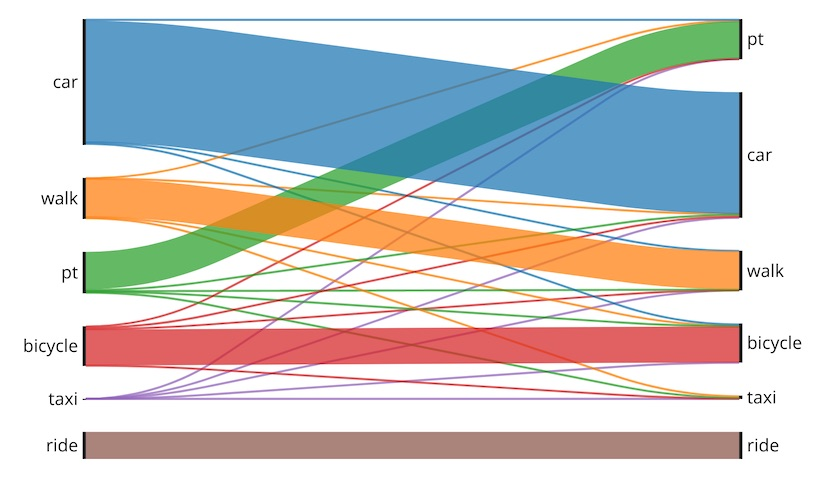
\includegraphics[width=0.8\textwidth]{assets/sankey.jpg}
  \caption{Mode shifts depicted as a Sankey diagram}
\end{figure}

Sankey diagrams are great for showing the shift between two states; for example
mode share shift from alt. A to alt. B. You see these a lot in politics
after a parliamentary election, to show the change in the number of
seats for each party.

\hypertarget{usage}{%
\subsection{Usage}}

Standalone: a file named \texttt{sankey-*.yml} must be present in
working folder. Each yml file matching that pattern will produce a
separate Sankey diagram.

Dashboard: Each panel is defined inside a \textbf{row} in a
\texttt{dashboard-*.yaml} file.

\begin{itemize}
\tightlist
\item
  Use panel \texttt{type:\ sankey} in the dashboard configuration.
\end{itemize}

\textbf{sankey-example.yml}

\begin{lstlisting}
  # only the csv line is required, but title and description help your viewers
  type: sankey
  csv: modeshares.csv
  title: Sankey Demo
  description: Erster Schritt!
\end{lstlisting}

\hypertarget{sankey-csv-file-format}{%
\subsection{Sankey CSV File format}\label{sankey-csv-file-format}}

Header line can contain labels but is CURRENTLY IGNORED

\begin{itemize}
\tightlist
\item
  Column 1: `From' category
\item
  Column 2: `To' category. These are not required to match the labels in
  column 1.
\item
  Column 3: Value
\item
  All other columns ignored
\end{itemize}

\textbf{Example:}

\begin{lstlisting}
from;to;number of trips (sample size); average change [sec]

car;car;748552;4.851276865
walk;walk;236111;0.064274854
walk;car;1644;-797.9385645
pt;ride;0;0
pt;bicycle;3167;-394.8995895
bicycle;walk;2276;925.78471

ride;bicycle;0;0
\end{lstlisting}
